\section{When replay pays off}
\label{sec:discussion}

\subsection{Analytical state-size projection}

Let \(N\) count trainable scalars, \(D\) count simultaneously
unresolved forks, and \(K\) count gradient events per edge. We
assume dense buffers and one full saved optimizer state per
fork. On the default spine, the \(D\) forks lie on a retained
path of \(D\) edges. We charge \(b_{\rm ID}\) bytes per event ID
to device storage in the projection. The measured driver kept
IDs on the host. In bytes, the phase state and tape together
cost \(8N+b_{\rm ID}KD\) for native or int32 replay and
\(16N+b_{\rm ID}KD\) for int64. Dense resident momentum SGD
costs \(8N(1+D)\), and resident AdamW costs \((12N+b_t)(1+D)\),
where \(b_t\) is the logical serialized size of its step counter.
These costs follow from the number of authoritative buffers and
their representation widths. Pinning the checkpoints places
the snapshot bytes in host memory and adds transfer time. In a
general tree with retained path length \(L\), the tape costs
\(b_{\rm ID}KL\) bytes and the checkpoint count still depends on \(D\).

With \(N=10^9\) trainable parameters and \(D=8\) unresolved
forks, the state terms \(8N\), \(8N(1+D)\), and \(12N(1+D)\)
give 8 GB for int32 DKD, 72 GB for dense momentum SGD, and 108 GB
for dense AdamW. These are algebraic estimates in decimal GB,
excluding event IDs and step counters, with no measured run at
this scale.

At positive depth, int32 uses fewer state-and-ID bytes than
resident momentum SGD if \(8N>b_{\rm ID}K\). Under that condition,
int64 crosses over at \(D>8N/(8N-b_{\rm ID}K)\). The model
excludes activations, gradients, arithmetic workspaces, allocator
reservations, checkpoint copies in flight, fixed backbone memory,
and the external event corpus. Runtime requires a separate measurement.
The first measured int64 allocation win against GPU SGD occurred
at tested depth \PthreeIntHighFirstSgdWin{}. The grid in
Table~\ref{tab:branching} skips the depth between that observation
and the first modeled win. Reducing the trainable subset cuts
checkpoint storage in proportion to the saved state even when
the forward pass still uses the complete backbone.

\begin{figure}[tbp]
  \centering
  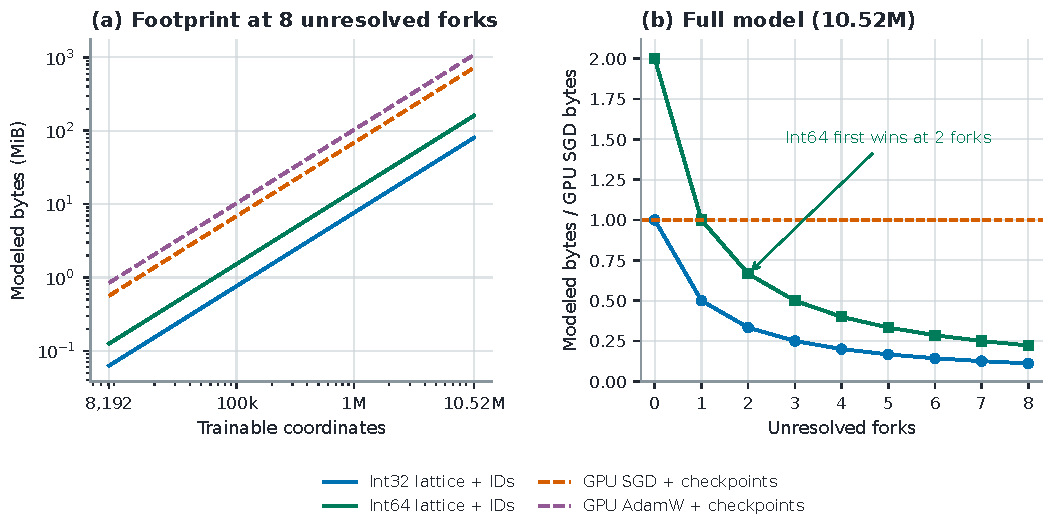
\includegraphics[width=\linewidth]{figures/fig4_scale_crossover.pdf}
  \caption{Analytical projections for dense optimizer state and
  identifier storage. The projections use \(K=\PthreeStepsPerEdge{}\)
  gradient events per edge and \(b_{\rm ID}=\PthreeEventIDBytes{}\)
  bytes per event ID, charged
  to the device here and stored on the host in the measurements.
  The AdamW counter uses \(b_t=\PthreeAdamCounterBytes{}\) logical
  serialized bytes. At the full-model size, int64 first strictly
  beats dense SGD in modeled storage at \(D=2\). At \(D=1\) its
  modeled state and tape use \PthreeSingleForkTapeBytes{} more
  bytes than SGD. Int64 first beats SGD in \emph{measured allocator}
  bytes at the tested depth \PthreeIntHighFirstSgdWin{}.
  These curves count state and IDs only.}
  \label{fig:scaling}
\end{figure}

\subsection{Limits and practical conditions}

Replaying a speculative update requires a reproducible gradient
tape and a rewind interval within the numerical range. The
integer inverse can return the exact starting state even after
rounding removes a forward kick. For that reason, an evaluation
needs to check forward utility and representation failures
alongside reverse error. The timing of actionable feedback also
matters. Rewind can recover accuracy when the signal arrives
after a damaging update, while an early warning can avoid
committing that update. The exploratory skip policy needs a
fresh comparison that includes the cost of scoring the warning.

The strongest checkpoint comparator depends on both the size
and location of the saved state. Replay reduced peak GPU
allocation relative to dense resident checkpoints in the
full-model tests. At the common deep-search solve rate, pinned-host
SGD took less time, and a small trainable head further reduced
the checkpoint size in the exploratory control.

The precision results depend on deterministic replay, fixed
scales, and lossless initialization on the tested grid. The
experiments leave open localization of unknown corruption
onsets, conversion of arbitrary pretrained checkpoints,
unrestricted branching, and generalization to other model or
task families. The retention results apply to the tested Fisher
estimators, interventions, validation grids, and adaptation
constraints. The systems measurements come from one GPU and
short procedural inputs. Appendix~\ref{app:reproducibility} gives the
scope of the backend checks and post-hoc reruns. The state-size
projection follows from the assumptions above.
